\documentclass[a4paper,10pt]{article}
\usepackage[utf8]{inputenc}
\usepackage{amsmath}
\usepackage{graphicx}
\usepackage{epstopdf}
\usepackage{textcomp}

\DeclareMathOperator*{\argmax}{arg\,max}
\DeclareMathOperator*{\argmin}{arg\,min}

%opening
\title{Tomografía óptica usando la ecuación independiente del tiempo de transferencia radiativa}
\author{A. Mendez}

\begin{document}

\maketitle

\begin{abstract}
El presente estudio consiste de dos partes. El objetivo general consiste
en introducir y testear experimentalmente un algoritmo novedoso de 
generación de imagenes de tomografía óptica basado en la ecuación de 
transferencia radiativa. Usar la ecuación de transferencia radiativa
en lugar de la ecuación de difusión permite considerar el medio 
altamente dispersivo que contiene regiones de vacío que tienen 
coeficientes bajos de absorción y dispersión.
En la parte I nos concentramos en los detalles de la descripción y 
evaluación de un modelo forward que describe con precisión la propagación 
de fotones en tales medios. En la parte II nos concentramos en la 
inclusión de este modelo en un esquema iterativo de reconstrucción de 
imágenes basado en modelos (MOBIIR por sus siglas en inglés). Usando el 
esquema MOBIIR se puede determinar la distribución espacial de las 
propiedades ópticas dentro de los medios altamente dispersivos a partir 
de mediciones adquiridas en la superficie del medio. Se presentarán el 
sustento matemático y numérico para la reconstrucción del algoritmo,
especialmente el esquema de diferenciación adjunta para el cálculo del
gradiente. El código es testeado con data experimental usando 
tissue-phantoms que contienen regiones rellenadas con agua o de vacío.

\end{abstract}

\section{Introducción}

La tomografía óptica (OT), también denominada tomografía óptica difusa 
(DOT), o tomografía de migración de fotón (PMT), ha realizado
considerables avances en los años recientes. En esta técnica la luz de
infrarojo cercano en la región de longitud de onda de aproximadamente
650nm$<\lambda<$900nm es utilizada para iluminar medios altamente
dispersivos. Basándose en mediciones de intensidades transmitidas y/o
reflejadas en la superficie de un medio, se intenta reconstruir la
distribución espacial de las propiedades ópticas (por ejemplo, el
coeficiente de absorción $\mu_a$ y el coeficiente de dispersión $\mu_s$)
dentro del medio. A pesar de que se pueden encontrar problemas 
similares en diferentes áreas científicas, yendo desde la oceonografía
hasta las ciencias atmosféricas, la astronomía y la física de neutrones,
los recientes avances en tomografía óptica han sido aportados por las
aplicaciones en la óptica biomédica. Este campo está enfocado en el uso 
de la luz visible y cercana al infrarojo para el diagnóstico y 
tratamiento de tejidos biológicos. Existen ejemplos de monitoreo óptico 
de oxigenación de sangre, detección de hemorragias cerebrales, mapeo
functional de actividad cerebral y diagnóstico de la enfermedad de
Alzheimer, artritis reumoidal, o cancer. Estas aplicaciones se basan en 
el hecho de que varios procesos de la enfermedad y la mayoría de los
cambios fisiológicos afectan las propiedades ópticas de los tejidos 
biológicos. Las propiedades ópticas de interés son los coeficientes de 
absorción $\mu_a$, de dispersión $\mu_s$, y el factor de 
anisotropía~$g$, o una combinación de ellos. Las diferencias en estas
propiedades ópticas entre tejidos sanos y patológicos proveen un 
contraste para esta tecnología de mapeo.

La mayoría de los grupos en esta área de investigación utilizan técnicas 
denominadas reconstrucción de imagen iterativo basado en modelos (MOBIIR).
Estas técnicas implementan modelos hacia adelante que provee predicciones
en las lecturas del detector basándose en la estimación de la distribución
espacial de estas propiedades ópticas dentro del medio. Las lecturas
predichas por el detector son comparadas con data experimental usando 
una función objetivo definida de manera apropiada. La verdadera
distribución de las propiedades ópticas se determina actualizando
iterativamente las predicciones y realizando nuevos cálculos hacia
adelante con estas propiedades ópticas actualizadas hasta que los datos
predichos coinciden con las lecturas del detector. La distribución final
de las propiedades ópticas se muestra como una imagen.

Es claro que la calidad de la imagen reconstruida depende fuertemente de 
la precisión del modelo hacia adelante. Si el modelo hacia adelante no 
describe de forma precisa la propagación de los fotones dentro del 
medio, el esquema de reconstrucción basado en el modelo fallará. Hasta
ahora, la mayoría de los algoritmos se basan en la validez de la
aproximación de difusión de la ecuación de transferencia de radiación.
Mientras que en la mayoría de los casos, ésta es una buena aproximación
para describir la propagación de luz en tejidos biológicos, varios
investigadores han probado experimental y teoréticamente cuáles son los
límites de esta aproximación. Por ejemplo, se ha mostrado que la
aproximación de difusión falla cuando el medio contiene regiones de
absorción en los cuales el coeficiente de absorción no es mucho menor 
que el coeficiente de dispersión, o en regiones en las que la dispersión 
y absorción son muy bajas, las llamadas regiones de simil-vacío. 
Medios turbios que contienen áreas tipo simil-vacío tienen un rol
importante en varias aplicaciones de mapeo biomédicos. Por ejemplo, los
tejidos cerebrales altamente dispersivos están encapsulados en una capa 
de fluido cerebroespinal casi transparente, el cual tiene un coeficiente
de dispersión y de absorción muy bajo. Cómo es que estas capas afectan 
la propagación de la luz ha sido recientemente objeto de muchos estudios 
y discusiones. 

\section{Métodos numéricos}

El transporte de fotones en medios dispersivos puede describirse a 
través de la ecuación independiente del tiempo de transferencia 
radiativa, dada por
\begin{equation}
 \omega\nabla\Psi(\mathbf{r},\omega)+(\mu_a+\mu_s)\Psi(\mathbf{r},\omega)
 =S(\mathbf{r},\omega) + 
 \mu_s\int_0^{2\pi}p(\omega,\omega')\Psi(\mathbf{r},\omega')\,d\omega'\,.
\end{equation}
La cantidad fundamental en la teoría de transporte radiativo es la
radiancia $\Psi(\mathbf{r},\omega)$ en la posición espacial 
$\mathbf{r}$, sobre un unidad de ángulo sólido $\omega$, con unidades 
W cm$^{-2}$ sr$^{-1}$. La integral de la radiación sobre todos los 
ángulos $\omega$ en el punto $\mathbf{r}$ define la fluencia (densidad de 
energía) $\Phi(\mathbf{r})$:
\begin{equation}
 \Phi(\mathbf{r})=\int_{2\pi}\Psi(\mathbf{r},\omega)\,d\omega\,.
\end{equation}
Otras cantidades incluidas en la ecuación de transporte son los 
coeficientes de dispersión $\mu_s$ y de absorción $\mu_a$, ambos dados 
en unidades de cm$^{-1}$, y la función de fase de dispersión 
$p(\omega,\omega')$. La función más comunmente usada es la función de dispersión de Henyey-Greennstein
\begin{equation}
 p(\cos\theta)=\frac{1-g^2}{2(1+g^2-2g\cos\theta)^{3/2}}\,
\end{equation}
donde $\theta$ es el ángulo entre las dos direcciones $\omega$ y 
$\omega$'. El factor $g$ se denomina factor de anisotropía y es utilizado 
para caracterizar la distribución angular de dispersión.


\section{Tissue phantoms y el set up experimental}

\subsection{Tissue phantoms}

Los tissue phantoms están compuestos de epoxy de resina claro en las que
se mezclaron monoesferas de dioxidos de silicio (SiO$_2$) y tinta. Las 
propiedades dispersivas fueron ajustadas variando la concentración de las
monoesferas, mientras que las propiedades de absorción fueron controladas
a través de la concentración de la tinta. El factor $g$ podría ser variado 
usando 

\begin{figure}
 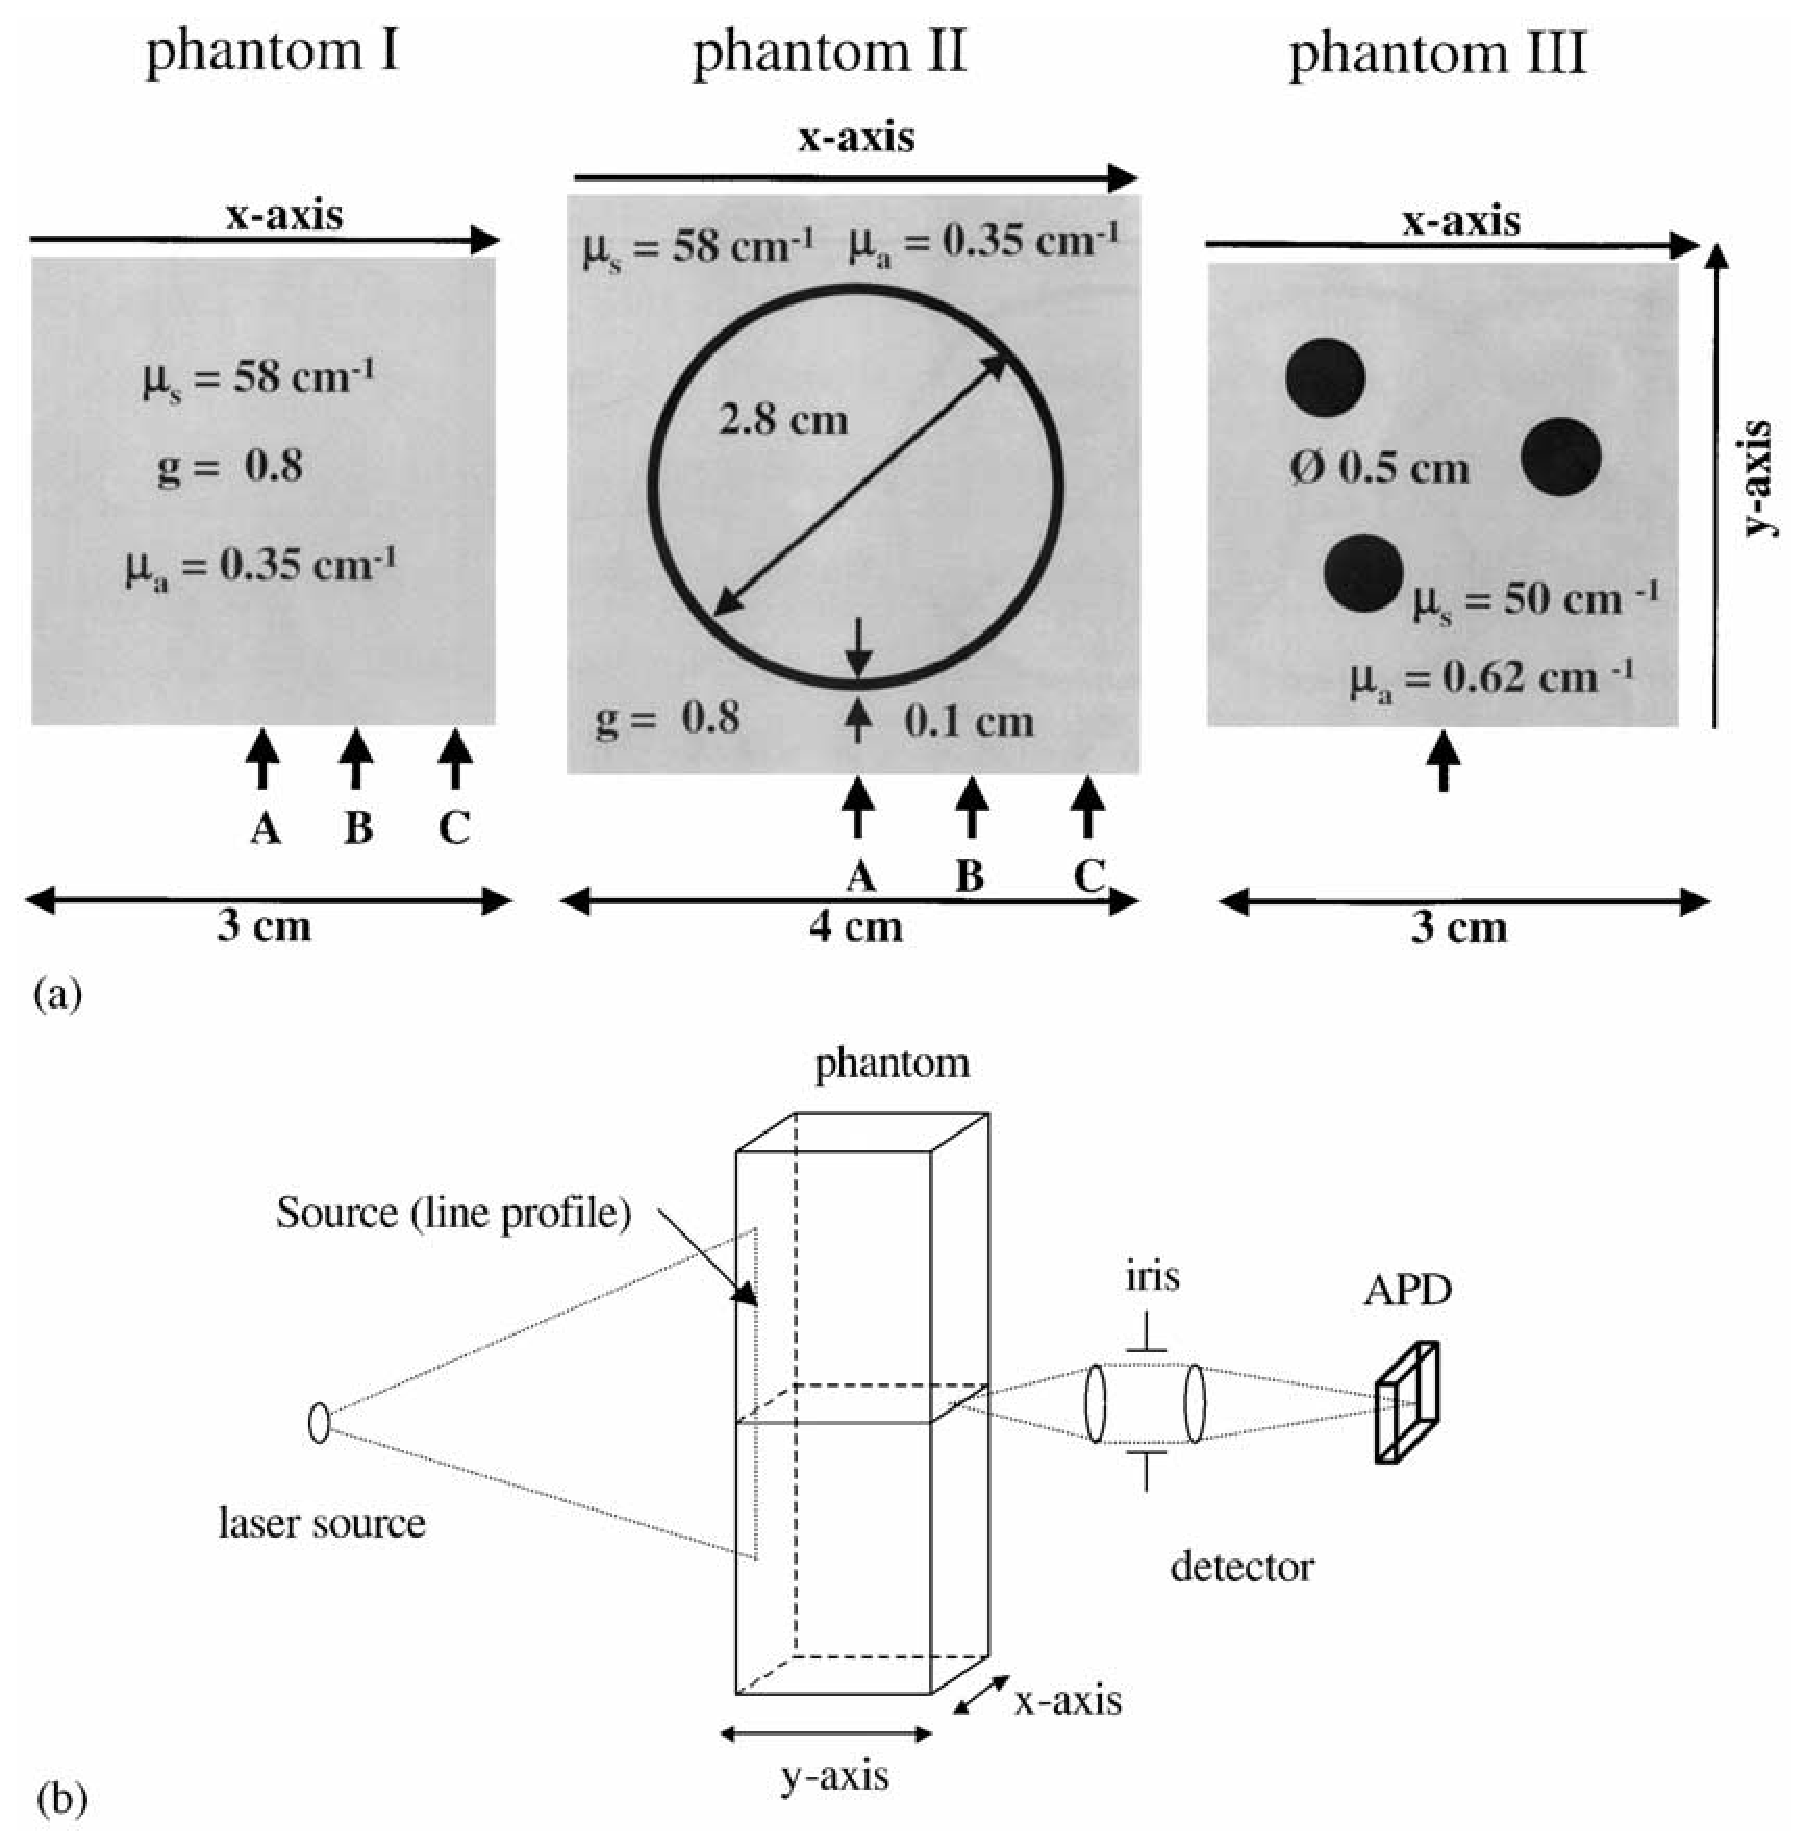
\includegraphics[width=0.9\textwidth]{fig1.eps}
\end{figure}


\subsection{Fuente de luz}

Los phantoms fueron iluminados con luz cercana al infrarojo de un láser
de diodo a $\lambda=678$nm. Dado que los phantoms son tridimensionales,
pero los cálculos son bidimensionales, fue necesario proveer un eje $z$
independiente. Esto fue alcanzado iluminando el phantom con una fuente 
de luz lineal extendida a lo largo del eje $z$. La fuente de luz obtenida 
a partir de un diodo láser con un ángulo de emisión de 20\textdegree a lo 
largo del eje $z$, mientras que el haz fue colimado a lo largo del eje 
$x$. De esta forma, la fuente de luz consistió en una línea de 6 cm de 
longitud y un ancho de 0.1 cm sobre la superficie del phantom. La potencia
de la fuente aplicada a un área de 0.001 cm$^2$ fue de 0.2$\pm$0.01 mW. 
Se tomaron medidas a lo largo del eje $x$.



\subsection{Sistema de detección de la luz}
La medición de la fluencia $\Phi$ se utilizó un photodiodo de avalancha
APD.



\end{document}
